\chapter{Representaci\'on y an\'alisis gr\'afico}

\section{Introducci\'on}

En este cap\'itulo, se aprender\'a c\'omo representar datos experimentales de manera efectiva mediante gr\'aficos. Se abordar\'an t\'ecnicas para la creaci\'on de gr\'aficos claros y comprensibles, as\'i como para el an\'alisis de datos a trav\'es de regresi\'on lineal y la interpretaci\'on de pendientes e intersecciones.

Para el cient\'ifico, analista de datos o persona con la responsabilidad  de escribir documentos t\'ecnicos es importante que desarrolle competencias en las t\'ecnicas de visualizaci\'on de datos. Las presentaciones con gr\'aficos deben ser claras, atractivas y sobre todo convincentes, muchas veces deben lograr traducir cantidades num\'ericas a ideas que permitan hacer extrapolaciones y proyecciones a situaciones futuras. Las t\'ecnicas de visualizaci\'on de datos termina siendo algo que se aprende con el oficio, con el d\'ia a d\'ia del trabajo de investigaci\'on y pocas veces se ense\~na en las universidades

El prop\'osito de este cap\'itulo es hacer una peque\~na introducci\'on sobre visualizaci\'on de datos y como usarlos en el an\'alisis de los datos experimentales. 

\section{Tabulaci\'on de datos y resultados}

La F\'isica es una ciencia experimental y cuantitativa, depende del trabajo de laboratorio donde se tendr\'a la necesidad de medir magnitudes y procesar datos.

Es una norma b\'asica que dichos datos deben ser presentados en forma clara y ordenada, y la mejor forma para lograr esto es ubicar los datos en tablas, donde se destinen diferentes columnas a cada conjunto de datos. Conocer en qu\'e consiste la tabulaci\'on de los datos y c\'omo hacerlo correctamente puede resultar de gran ayuda a la hora de realizar las diferentes etapas de  procesamiento y visualizaci\'on, facilita considerablemente la comprensi\'on, el an\'alisis y la interpretaci\'on de los datos para llevar a cabo comparaciones y obtener conclusiones v\'alidas. 

Las ventajas de este proceso de tabulaci\'on son las siguientes:
\begin{enumerate}
\item Cumplir con condiciones de claridad y orden.
\item Facilitar la lectura y la comprensi\'on de los datos.
\item Reducir las posibilidades de equivocaci\'on al tomar valores para calcular.
\end{enumerate}

Las Tablas deben ser lo m\'as autocontenidas posibles, sus t\'itulos y  leyendas deben ser suficiente para explicar su contenido. Las leyendas de tablas y figuras deben ser m\'as que una simple descripci\'on. Deben generar una reflexi\'on una conclusi\'on al presentar la tabla o figura. En textos cient\'ificos las tablas deben ser referidas desde el texto (ver Tabla \ref{ejetabla1}). Si no se hace referencia a una tabla en particular, \'esta se considera in\'util para el art\'iculo y debe ser eliminada.

La confecci\'on de tablas de valores no se limita necesariamente a los datos que se recogen directamente en el trabajo experimental, sino que puede extenderse a los resultados de efectuar operaciones con dichos datos. Adem\'as en dichas tablas, deben disponerse columnas para colocar en ellas el error con el cual dichas magnitudes han sido medidas, siempre que este sea diferente en cada medici\'on.

Las tablas en las que se recopilan y se organizan los datos deben contar con las siguientes partes:
\begin{itemize}
\item T\'itulo de la tabla: debe ser breve, conciso y claro.
\item Contenido de la tabla:  deben aparecer las magnitudes con sus respectivos nombres y unidades, preferiblemente  en el mismo sistema de unidades.
\item N\'umero de la tabla.
\item Notas explicativas: hacer referencia a la fuente de los datos, explicaci\'on de las abreviaturas, consideraciones a tener en cuenta, etc. 
\end{itemize}

Como ejemplo de lo dicho anteriormente se presenta una tabla de valores obtenida en una experiencia de movimiento rectil\'ineo uniformemente acelerado, ver tabla \ref{ejetabla1}

\begin{table}[!h]
\centering
\caption{Velocidad de carrera sobre 200$ \mathrm{~m}$ y distancia de salto de longitud  de un grupo de personas seleccionadas al azar.}
\begin{tabular}{ccc}
\hline Participante & Velocidad $\left(\mathrm{ms}^{-1}\right)$ & Distancia $(\mathrm{m})$ \\ \hline \hline 
1 & 10.53 & 2.38 \\
2 & 11.16 & 1.83 \\
3 &  9.54  & 2.04 \\
4 & 15.77 & NA\footnote{El participante 4 no pudo realizar el salto de longitud  por razones m\'edicas} \\
5 & 12.82 & 1.74 \\
& & \\
Total & 59.82 & 7.99 \\
Promedio & 11.964 & 1.997 \\
\hline
\end{tabular}
\label{ejetabla1}
\end{table}


\section{Representaciones  gr\'aficas}

La representaci\'on de gr\'aficas o la visualizaci\'on de datos es una t\'ecnica art\'istica que permite transmitir el conocimiento cient\'ifico. Con la visualizaci\'on de datos se debe transmitir de manera precisa la informaci\'on cient\'ifica relevante sin distorsionar su contenido. No debe contener informaci\'on falsa ni err\'onea. Es necesario que la visualizaci\'on sea agradable desde el punto de vista est\'etico, si las figuras se muestran con colores poco arm\'onicos, elementos visuales engorrosos traer\'a como consecuencia que el espectador no pueda interpretar la figura de manera correcta. 

En muchos casos, una acertada visualizaci\'on de datos  permite determinar valores que no han sido obtenidos experimentalmente, como son:
\begin{enumerate}
\item Valores entre puntos experimentales (proceso de Interpolaci\'on).
\item Valores fuera del intervalo experimental (proceso de Extrapolaci\'on).
\item Valores de los par\'ametros constantes de la funci\'on matem\'atica usada.
\end{enumerate}

En la figura \ref{estilosfig}\footnote{Tomada de: \url{https://clauswilke.com/dataviz/}.} podemos ver algunos ejemplos  de c\'omo hacer una buena visualizaci\'on y otras como ejemplos de c\'omo no hacerla.  Una figura  que muestre problemas est\'eticos pero que cumple con su funci\'on de ser clara e informativa es una figura que podr\'iamos llamar ``fea''. Una figura ``mala'' es aquella que es poco clara, confusa, complicada, enga\~nosa, mientras que una figura ``incorrecta'' es aquella que presenta informaci\'on err\'onea, presenta inconsistencias matem\'aticas que inevitablemente llevar\'a a una interpretaci\'on equivocada de los datos.
\begin{figure}[h]
\begin{center}
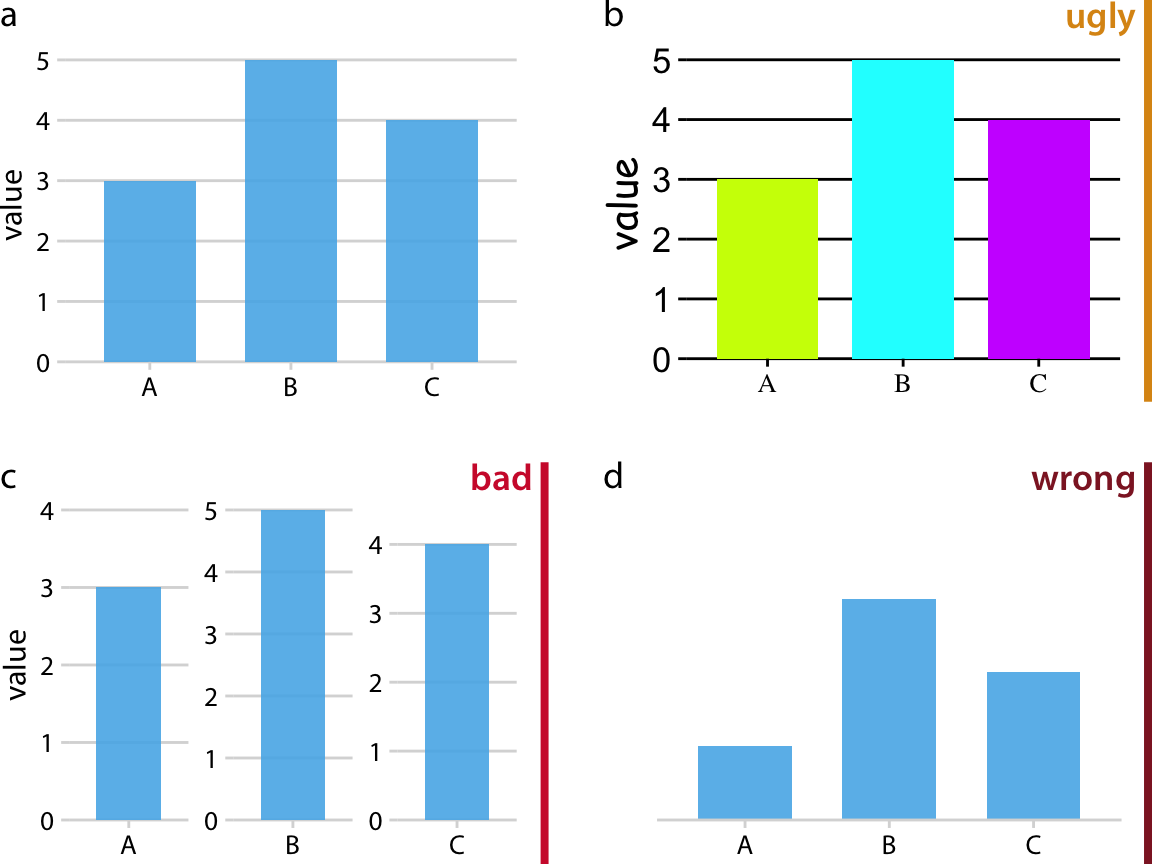
\includegraphics[height=2.5in,width=3.6in]{figuras/fig08}  
\caption{En (a) se muestra  un diagrama de barras para tres valores: A = 3, B = 5 y C = 4;  es una representaci\'on sencilla y entendible. (b) es una versi\'on fea de la parte (a), aunque el gr\'afico es t\'ecnicamente correcto, es est\'eticamente desagradable, con colores innecesarios, una cuadr\'icula de fondo absurda y un texto con tipos de letra y tama\~nos diferentes. (c) es una mala versi\'on de la parte (a), en el eje $y$ cada barra tiene  su propia escala y adem\'as est\'an desalineadas, por lo tanto es una gr\'afica enga\~nosa. (d) es una versi\'on incorrecta de la parte (a), como el eje $y$ no pose escalas no es posible determinar sus valores num\'ericos.}
\label{estilosfig}
\end{center}
\end{figure}


Cuando se grafican valores experimentales o magnitudes calculadas se debe considerar:

\subsection{Ejes de coordenadas}

En muchas casos, cuando se quiere visualizar datos se necesita definir escalas que permitan posicionar los datos en un gr\'afico. En gr\'aficos 2D se necesitan dos n\'umeros para especificar un punto de manera un\'ivoca, es decir, dos escalas de posici\'on. Estas dos escalas suelen ser los ejes $x$ (eje horizontal o eje de las abscisas) y el eje $y$ (eje vertical o eje de las ordenadas), es lo generalmente  se denomina el sistema de coordenadas.

\begin{enumerate}
\item En los ejes deben aparecer claramente las magnitudes, s\'imbolo o letra, que en ellos se representan y sus unidades de medida correspondientes

\item En los ejes s\'olo deben colocarse los valores m\'as representativos de la escala escogida.

\item En general, es conveniente que el origen aparezca en el gr\'afico, pero no siempre es necesario que la intersecci\'on de los dos ejes corresponda al punto cero; en este caso las escalas pueden desplazarse cuando los datos experimentales est\'an en un intervalo que as\'i lo requiera.

\item La variable independiente, cuyo valor lo asigna a conveniencia el experimentador, se representa sobre el eje $x$ horizontal y la variable que depende de ese valor asignado se coloca sobre el eje $y$ vertical.
\end{enumerate}


\subsection{Selecci\'on de escalas}
La escogencia de las escalas a utilizar es un problema si no se tiene cuidado al considerar factores como: el tama\~no del conjunto de datos, las divisiones sobre cada eje, la relaci\'on entre los errores experimentales y los valore m\'inimos elegidos en las escalas. 

Las escala no deben ser muy peque\~na, ya que en este  caso se  pueden agrupar exageradamente los puntos en una regi\'on de la gr\'afica (ver figura \ref{escala1}). Tampoco deben elegirse escalas grandes que exageran la precisi\'on.
\begin{figure}[h]
\begin{center}
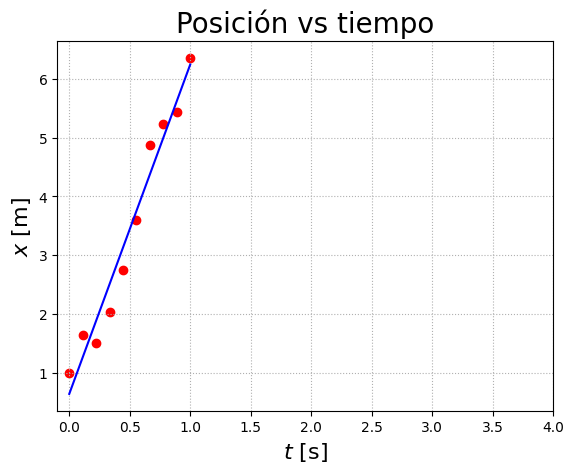
\includegraphics[height=2.5in,width=3.6in]{figuras/fig09}  
\caption{Muy mala selecci\'on de las escalas.}
\label{escala1}
\end{center}
\end{figure}

Una gr\'afica puede requerir  tener dos ejes que representan dos unidades diferentes, por ejemplo Temperatura en $^\circ$C vs Tiempo en s.  Estirar o comprimir los ejes obedecer\'a a las razones que necesitemos resaltar, una gr\'afica alta y estrecha enfatiza el cambio a lo largo del eje $y$ y una corta y ancha hace lo contrario. Lo ideal es elegir una relaci\'on de aspecto que garantice que las diferencias importantes de posici\'on sean perceptibles.

Por otro lado, si los ejes $x$ y $y$ se miden en las mismas unidades, entonces las separaciones de la cuadr\'icula para los dos ejes deben ser iguales, de forma que la misma distancia a lo largo del eje $x$ o $y$ corresponda al mismo n\'umero de unidades de datos.

Los sistemas de coordenadas cartesianos son sistemas de coordenadas lineales y aunque 
suelen proporcionar una representaci\'on precisa de los datos, hay situaciones en las que se prefiere utilizar escalas no lineales. En una escala no lineal, a un espaciado uniforme en las unidades de datos le corresponde un espaciado desigual en la visualizaci\'on o, contrariamente, a un espaciado uniforme en la visualizaci\'on le corresponde un espaciado desigual en las unidades de datos.

La escala no lineal m\'as utilizada es la escala logar\'itmica o escala logar\'itmica abreviada, estas escalas  son lineales en la multiplicaci\'on, de forma que un paso unitario en la escala corresponde a una multiplicaci\'on con un valor fijo. Para crear una escala logar\'itmica, debemos realizar una transformaci\'on logar\'itmica de los valores de los datos y exponenciar los n\'umeros que se muestran a lo largo de las l\'ineas de la cuadr\'icula del eje.


\subsection{Ubicaci\'on de los puntos}

Los valores experimentales no deben ser graficadas s\'olo como un solo punto, se debe representar adem\'as el error absoluto con el cual se obtuvo dicho valor. Para ello se usan: cuadrados, rect\'angulos, barras, cruces, etc. (ver figura \ref{barerror}). Si la escala escogida no permite representar el error absoluto, los valores experimentales se deben representar con una equis o una cruz. Las barras de error suelen representarse a lo largo de las direcciones $x$ y  $y$ en un gr\'afico de dispersi\'on.

En las figuras 2D sencillas, las barras de error tienen una ventaja importante sobre las representaciones m\'as complejas de la incertidumbre ya que se pueden combinar con muchos otros tipos de gr\'aficos. Por lo tanto, las barras de error resultan ser la representaciones m\'as sencillas para mostrar cantidades con incertidumbre sobre todo en las gr\'aficas de barras. 

Cada conjunto debe ser representado por un s\'imbolo diferente, por ejemplo: $\times, \Delta, \odot,+$ e identificar luego cada curva. La recta o curva que siguen los puntos se debe trazar de un modo que la funci\'on sea lo m\'as representativa posible del comportamiento de las magnitudes que caracterizan el fen\'omeno  en estudio.
\begin{figure}[h]
\begin{center}
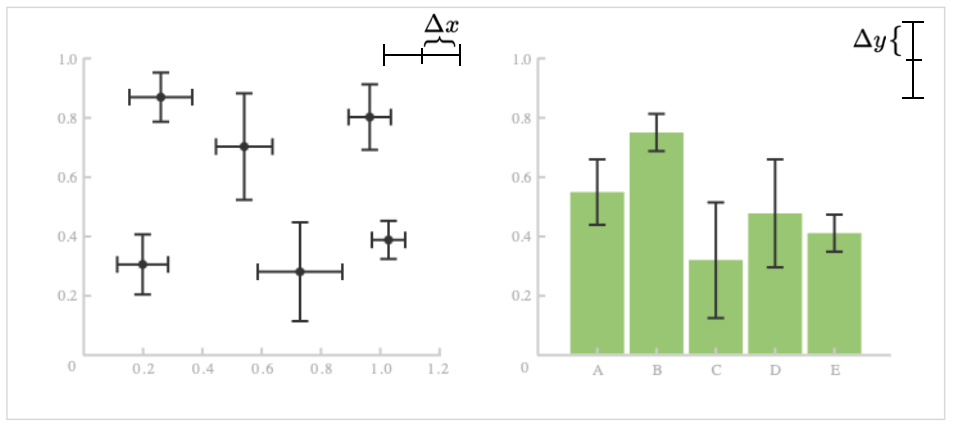
\includegraphics[height=2.2in,width=4.6in]{figuras/fig11}  
\caption{Representaci\'on de puntos experimentales con barras de error.}
\label{barerror}
\end{center}
\end{figure}


\section{Trazado de una recta}

En algunos experimentos las magnitudes f\'isicas pueden variar linealmente, como es el caso de la deformaci\'on y la fuerza en la ley de Hooke $(F = -kx)$. Al realizar el experimento y graficar resulta  un conjunto de puntos que corresponde a un comportamiento lineal. 

El experimentador tiene que buscar ahora la mejor estrategia  para trazar la mejor recta que pasa por entre los puntos experimentales.

Los m\'etodos estad\'isticos demuestran que, siempre que la dispersi\'on de los puntos experimentales  se deba a los errores casuales de medici\'on, la mejor recta pasar\'a por el centroide de los puntos experimentales, que es el punto con las coordenadas
$(\bar{x}, \bar{y})$, en donde $\bar{x}$ y $\bar{y}$  son los  valores medios de las coordenadas $x$ y $y$ respectivamente.
\begin{equation}
\begin{aligned}
\bar{x} & =\frac{1}{n}{\sum_{i=1}^n x_i} \\
\bar{y} & =\frac{1}{n}{\sum_{i=1}^n y_i}
\end{aligned}
\end{equation}


Para ajustar la recta al conjunto de puntos experimentales, se emplear\'an los siguientes m\'etodos:

\subsection{M\'etodo gr\'afico}
Este m\'etodo es un m\'etodo artesanal, y consiste en buscar sobre la gr\'afica la mejor recta que pase  por el centroide y la mayor\'ia de los puntos experimentales. Aquellos puntos que queden por fuera de esta recta deben estar distribuidos en lo posible con igual peso a ambos lados de la curva.

Como sabemos, la ecuaci\'on de una recta es:
$$
y=m x+b
$$
donde:
\begin{itemize}
\item $m$ es la pendiente de la recta, calculada a partir de las coordenadas de dos puntos sobre la recta, necesariamente no tienen que corresponder a valores experimentales.
$$
m=\frac{\left(y_2-y_1\right)}{\left(x_2-x_1\right)} \frac{\text { unidad de } y}{\text { unidad de } x}
$$
\item  $b$ es el corte de la recta con el eje de las ordenadas en $x=0$.
\end{itemize}

El error absoluto para $m$ y $b$ viene dado por la lectura de la posici\'on de los puntos sobre el gr\'afico, es decir en funci\'on de la apreciaci\'on de la escala en el eje respectivo.


\subsection{M\'etodo de los m\'inimos cuadrados}

El m\'etodo de los m\'inimos cuadrados es uno de los m\'etodos estad\'isticos m\'as usados para determinar la recta que mejor represente la tendencia de un conjunto de puntos experimentales.

Si la dispersi\'on de los puntos experimentales es debida solo a los errores casuales en las mediciones, la mejor recta ser\'a aquella para la cual la suma de los cuadrados de las distancias $\left(y_i-y_0 \right)$ sea un m\'inimo, ver figura 4.4. Es por esto que, a este m\'etodo se le llama m\'etodo de los m\'inimos cuadrados.

Consideremos una relaci\'on lineal entre dos magnitudes f\'isicas $y$ y $x$ de la forma:
$$
y=m x+b
$$

Donde $y$ es la variable dependiente y $x$ es la variable independiente, en nuestro caso la magnitud controlada por el experimentador. Como ya se ha dicho anteriormente, los valores de esas magnitudes tendr\'an sus correspondientes errores, determinados por los m\'etodos ya se\~nalados. 

La desviaci\'on de un valor cualquiera $y_i$ determinado experimentalmente con respecto a su valor $y_0$ en la recta, ser\'a:
\begin{equation}
\Delta y_i=y_i-y_0=y_i-\left(b+m x_i\right)
\label{deltay}
\end{equation}

Ahora se puede enunciar el principio b\'asico de este m\'etodo, el cual dice que:

La mejor recta que puede ser trazada entre esos puntos, es aquella para la cual la suma de los cuadrados de las desviaciones $\Delta y_i$ de los datos experimentales, con respecto a esa recta, es m\'inima.
$$
\sum_{i=1}^n\left(\Delta y_i\right)^2=\sum_{i=1}^n \left[y_i-b-m x_i \right]^2
$$
donde $n$ es el n\'umero de pares de valores de $y$ y $x$.

Ya que la condici\'on exigida es la de minimizar la suma anterior, entonces los par\'ametros $m$ y $b$ deben ajustarse para cumplir con esta condici\'on. Ello se logra calculando las derivadas parciales de la suma con respecto a $m$ y con respecto a $b$, e igual\'andolas a cero.
$$
\begin{aligned}
& \frac{\partial\left[\sum\left(\Delta y_i\right)^2\right]}{\partial b}=
\sum_{i=1}^n\frac{\partial\left(y_i-b-m x_i \right)^2}{\partial b} = 
\sum_{i=1}^n -2(y_i-b-m x_i)=0  \\
& \frac{\partial\left[\sum\left(\Delta y_i\right)^2\right]}{\partial m}=
\sum_{i=1}^n\frac{\partial\left(y_i-b-m x_i \right)^2}{\partial m} =
\sum_{i=1}^n -2x_i(y_i-b-m x_i)=0
&
\end{aligned}
$$

Por lo tanto, se debe resolver el sistema 
$$
\begin{aligned}
&  \sum_{i=1}^n y_i - \sum_{i=1}^nb - \sum_{i=1}^n m x_i = 0  &\,\, \Rightarrow \,\,&
 nb + m \sum_{i=1}^n  x_i = \sum_{i=1}^n y_i  \\
&  \sum_{i=1}^n y_ix_i - \sum_{i=1}^n bx_i -\sum_{i=1}^n  m x_i^2 =0 & \,\, \Rightarrow \,\,&
b \sum_{i=1}^n x_i  + m \sum_{i=1}^n   x_i^2 = \sum_{i=1}^n y_ix_i
\end{aligned}
$$
para $m$ y $b$. 

Utilizando la regla de Cramer
$$
\begin{aligned}
\Delta= 
{\left|\begin{array}{cc}
n & \sum x_i \\
\sum x_i & \sum x_i^2
\end{array}\right|} = n \sum x_i^2-\left(\sum x_i\right)^2 \,,
\end{aligned}
$$

$$
\begin{aligned}
& b=\frac{\left|\begin{array}{cc}
\sum y_i & \sum x_i \\
\sum x_i y_i & \sum x_i^2 
\end{array}\right|}{\Delta}=\frac{\sum x_i^2 \sum y_i-\sum x_i \sum x_i y_i}{n \sum x_i^2-\left(\sum x_i\right)^2} \\ \\
& m=\frac{\left|\begin{array}{cc}
n & \sum y_i \\
\sum x_i & \sum x_i y_i
\end{array}\right|}{\Delta}=\frac{n\sum x_i y_i-\sum x_i \sum y_i}{n \sum x_i^2-\left(\sum x_i\right)^2}
\end{aligned}
$$

Por lo tanto:
\begin{eqnarray}
b &=&\dfrac{\sum\limits_{i=1}^n x_i^2 \sum\limits_{i=1}^n y_i-\sum\limits_{i=1}^n x_i \sum\limits_{i=1}^n x_i y_i}{n\sum\limits_{i=1}^n x_i^2-\left(\sum\limits_{i=1}^n x_i\right)^2} 
\label{emeyb1}\\
m &=&\dfrac{ n\sum\limits_{i=1}^n x_i y_i-\sum\limits_{i=1}^n x_i \sum\limits_{i=1}^n y_i}{n \sum\limits_{i=1}^n x_i^2-\left(\sum\limits_{i=1}^n x_i\right)^2}
\label{emeyb2}
\end{eqnarray}

De esta manera obtenemos la recta $f(x)=mx+b$ que mejor de aproxima a los puntos. 

N\'otese que los t\'erminos $\sum x_i^2$ y $\left(\sum x_i\right)^2$ no son lo mismo. Id\'entica observaci\'on se debe hacer para los t\'erminos $\sum\left(x_i y_i\right)$ y $\sum x_i \sum y_i$.

Es recomendable construir una tabla como \ref{tablamincua}, para as\'i ordenar la informaci\'on y facilitar los c\'alculos. Las cuatro sumas en la \'ultima l\'inea, son los valores necesarios para calcular $m$ y $b$. Los valores de $m$ y $b$ que se obtengan por el m\'etodo de los m\'inimos cuadrados, deber\'ian ser muy pr\'oximos a los obtenidos directamente utilizando el m\'etodo gr\'afico.
\begin{table}[h]
\begin{center}
\begin{tabular}{|c|c|c|c|}
\hline $y_i [\,\,]$ & $x_i [\,\,]$ & $x_i^2 [\,\,]$& $x_i y_i [\,\,]$ \\
\hline \hline $y_1$ & $x_1$ & $x_1^2$ & $x_1 y_1$ \\
\hline $\vdots$ & $\vdots$ & $\vdots$ & $\vdots$ \\
\hline $\vdots$ & $\vdots$ & $\vdots$ & $\vdots$ \\
\hline $y_n$ & $x_n$ & $x_n^2$ & $x_n y_n$ \\ \hline
\hline $\sum y_i$ &$\sum x_i $& $\sum x_i^2$ & $\sum x_i y_i$ \\
\hline
\end{tabular}
\end{center}
\caption{Tabla para facilitar el uso del  m\'etodo de m\'inimos cuadrados}
\label{tablamincua}
\end{table}


Actualmente es casi de rutina utilizar alguna herramienta computacional  que permite hacer los c\'alculos necesarios y los gr\'aficos para el ajuste de la recta. Aunque el uso de este m\'etodo no nos obliga a hacer el gr\'afico de la recta, por razones pedag\'ogicas, es conveniente hacerlo para as\'i observar m\'as claramente las desviaciones de los puntos experimentales con respecto a la recta calculada. 

Una vez obtenido los valores de $m$ y ${b}$, es necesario calcular sus errores correspondientes $\Delta m$ y $\Delta b$. Esto lo podemos hacer calculando las desviaciones est\'andar  de la pendiente y la ordenada al origen, calculadas a partir de la distribuci\'on de diferencias $\Delta y_i$, ecuaci\'on (\ref{deltay}),  respecto de la mejor l\'inea de ajuste. Sea  $S_y$  la  desviaci\'on est\'andar de $y$ respecto a la l\'inea recta obtenida por m\'inimos cuadrados:
\begin{equation}
S_y=\left[\frac{\sum\limits_{i=1}^n \left(y_i-b-m x_i\right)}{n-2}\right]^{\frac{1}{2}} \,.
\end{equation}

Para calcular estos valores de $\Delta m$ y $\Delta b$ se utilizan las siguientes expresiones:
\begin{eqnarray}
\Delta m & =\left[\frac{n}{n \sum\limits_{i=1}^n\left(x_i\right)^2-\left(\sum\limits_{i=1}^n x_i\right)^2}\right]^{\frac{1}{2}} S_y 
\label{Delm}\\
\Delta b & =\left[\frac{\sum\limits_{i=1}^n\left(x_i\right)^2}{n \sum\limits_{i=1}^n\left(x_i\right)^2-\left(\sum\limits_{i=1}^n x_i\right)^2}\right]^{\frac{1}{2}} S_y
\label{Delb}
\end{eqnarray}

La cantidad $S_y$ representa la llamada desviaci\'on est\'andar de $y$ respecto a la l\'inea recta obtenida.

Finalmente para calcular $S_y$ se puede utilizar como ayuda la tabla \ref{tablamincua2}
\begin{table}[h]
\begin{center}
\begin{tabular}{|c|c|c|c|}
\hline$x_i [\,\,]$ & $y_i [\,\,]$ & $y_i-m x_i-b$ & $(y_i-m x_i-b)^2$ \\
\hline \hline$x_1$ & $y_1$ & $y_1-m x_1-b$ & $\left(y_1-m x_1-b\right)^2$ \\
\hline$x_2$ & $y_2$ & $y_2-m x_2-b$ & $\left(y_2-m x_2-b\right)^2$ \\
\hline$\vdots$ & $\vdots$ & $\vdots$ & $\vdots$ \\
\hline$\vdots$ & $\vdots$ & $\vdots$ & $\vdots$ \\
\hline$x_n$ & $y_n$ & $y_n-m x_n-b$ & $\left(y_n-m x_n-b\right)^2$ \\ \hline
\hline & & & $\sum\limits_{i=1}^n \qquad \qquad \quad$ \\
\hline
\end{tabular}
\end{center}
\caption{Tabla para facilitar los c\'alculos de $S_y$.}
\label{tablamincua2}
\end{table}

\paragraph{Ejemplo 7.}

En un experimento sobre cinem\'atica un grupo de estudiantes mide los tiempos con los que se desplaza  un m\'ovil en un riel de aire. Lis tiempos son medidos en segundos usando un cron\'ometro de sensibilidad $S=0,01$ s. Un instrumento de mejor precisi\'on mide las velocidades con las que se desplaza el m\'ovil, este instrumento tiene una sensibilidad de $0,001$ m/s.  Los datos se muestran en la tabla \ref{datos1}.
\begin{table}[h]
\begin{center}
\begin{tabular}{|c|c|}
\hline $t_i \pm 0,01 (\mathrm{s})$ & $v_i \pm 0,01 (\mathrm{m/s})$  \\\hline \hline 
\hline $0,00$ & 1.00 \\
\hline $0,10$ & 1.64 \\
\hline $0,20$ & 1.51 \\
\hline $0,30$ & 2.03 \\
\hline $0,40$ & 2.75 \\
\hline $0,50$ & 3.59 \\
\hline $0,60$ & 4.87 \\
\hline $0,70$ & 5.23 \\
\hline $0,80$ & 5.44 \\
\hline $1,00$ & 6.37 \\
\hline
\end{tabular}
\end{center}
\caption{Mediciones de la velocidad de un cuerpo en funci\'on del tiempo}
\label{datos1}
\end{table}

Al graficar los datos anteriores se obtiene la figura
\begin{figure}[h]
\begin{center}
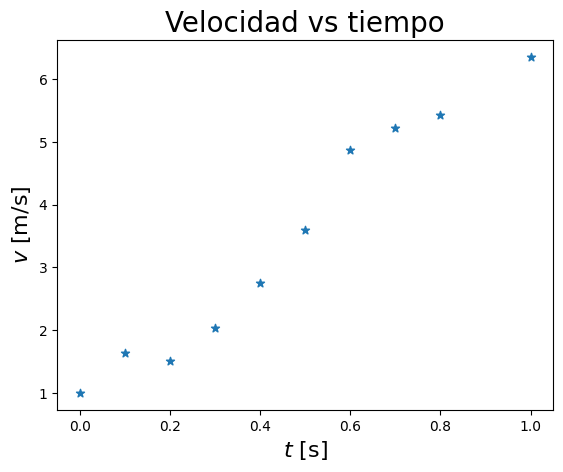
\includegraphics[height=2.5in,width=2.5in]{figuras/fig12}  
\caption{Gr\'afico de los datos $v$ vs $t$ de la tabla \ref{datos1}.}
\label{figdatos1}
\end{center}
\end{figure}

Es recomendable calcular las siguientes sumas:
$$
\begin{array}{c|c|c|c|c}
n&\sum_{i=1}^n t_i & \sum_{i=1}^n v_i   & \sum_{i=1}^n t_i^2  & \sum_{i=1}^n t_i v_i \\ \hline\hline 
10 & 4.60 & 34.43 & 3.04 & 21.3
\end{array}
$$
$$
\Delta=n\sum\limits_{i=1}^n t_i^2-\left(\sum\limits_{i=1}^n t_i\right)^2= 
10(3.04) - \left(4.60 \right)^2= 9.24 \,\, \mathrm{s}^2
$$
$$
b=\dfrac{\sum\limits_{i=1}^n t_i^2 \sum\limits_{i=1}^n v_i-\sum\limits_{i=1}^n t_i \sum\limits_{i=1}^n t_i v_i}{\Delta} =
\frac{(3.04)  (34.43) -(4.60) (21.3)}{9.24} = 0.724 \,\, \mathrm{m/s}
$$
$$
m =\dfrac{n \sum\limits_{i=1}^n t_i v_i-\sum\limits_{i=1}^n t_i \sum\limits_{i=1}^n v_i}{\Delta} =\frac{10(21.3)  -(4.60) ( 34.43)}{9.24}= 5.91\,\, \mathrm{m/s^2}
$$

Procedemos a calcular los errores 
$$
\begin{array}{c|c}
n& \sum\limits_{i=1}^n \left(v_i-b-m t_i\right)  \\ \hline\hline 
10 & 6.63 
\end{array}
$$
La desviaci\'on est\'andar de $y$:
$$
S_y=\left[\frac{\sum\limits_{i=1}^n \left(v_i-b-m t_i\right)^2}{n-2}\right]^{\frac{1}{2}}=
\left(\frac{6.63}{8}\right)^{\frac{1}{2}}=0.91 \,.
$$
y los errores 
$$
\begin{aligned}
\Delta m & =\left[\frac{n}{\Delta}\right]^{\frac{1}{2}} S_y = \left[\frac{10}{9.24}\right]^{\frac{1}{2}} (0.91)=0.95 \\
\Delta b & =\left[\frac{\sum\limits_{i=1}^n\left(t_i\right)^2}{\Delta}\right]^{\frac{1}{2}} S_y= 
\left[\frac{3.04}{9.24}\right]^{\frac{1}{2}} (0.91)= 0.52
\end{aligned}
$$

Por lo tanto nuestro resultado ser\'a:
$$
v=mt + b= 5.91 t + 0.724 \,\, \mathrm{m/s}
$$
donde $m=5.91 \pm 0.95$ y $b=0.72 \pm 0.52$.

En Python podemos hacer todos los casos anteriores, incluida la figura \ref{figdatos1}, pero primero debemos ingresar los datos
\begin{lstlisting}[language=Python]    
yn=  array([1.000, 1.64, 1.51, 2.03, 2.75, 3.59, 4.87, 5.23, 5.44, 6.37])
xn = array([0.00, 0.10, 0.20, 0.30, 0.40, 0.50, 0.60, 0.70, 0.80, 1.00])
\end{lstlisting}

La gr\'afica de la figura \ref{figdatos1} se obtiene a partir de las siguientes lineas de c\'odigo:
\begin{lstlisting}[language=Python] 
plt.scatter(xn, yn, marker='*')
plt.title(r'Velocidad vs tiempo', fontsize=20)
plt.xlabel(r'$t$ [s]', fontsize=16)
plt.ylabel(r'$v$ [m/s]', fontsize=16)
\end{lstlisting}

Para usar las ecuaciones (\ref{emeyb1})-(\ref{emeyb2}) hagamos primero los siguientes c\'alculos intermedios
\begin{lstlisting}[language=Python] 
#Se obtiene el valor de n (numero de datos)
n=len(xn)
#Las sumatorias necesarias 
Sum_x=sum(xn)
Sum_y=sum(yn)
Sum_xx=sum(xn**2)
Sum_xy=sum(xn*yn)
print(n,',', Sum_x, ',',Sum_y,',', Sum_xx,',', Sum_xy)
\end{lstlisting}
\begin{tcolorbox}[width=\textwidth,colback={ghostwhite}]   
{\small 
10 , 4.6 , 34.43 , 3.04 , 21.275
}
\end{tcolorbox} 

Y finalmente calculamos $b$ y $m$
\begin{lstlisting}[language=Python] 
# Se escriben las ecuaciones para b y m 
b=(Sum_xx*Sum_y-Sum_xy*Sum_x)/(n*Sum_xx-Sum_x**2)
m=(n*Sum_xy-Sum_x*Sum_y)/(n*Sum_xx-Sum_x**2)
print('m=',m, ',', 'b=',b)
\end{lstlisting}
\begin{tcolorbox}[width=\textwidth,colback={ghostwhite}]   
{\small 
m= 5.884415584415585 , b= 0.7361688311688325
}
\end{tcolorbox} 

Notemos lo diferente del valor de $m$ con respecto al obtenido anteriormente, esta diferencia obviamente se debe a que anteriormente fuimos haciendo redondeos en la operaciones. 

Veamos la recta y los datos
\begin{lstlisting}[language=Python] 
# La gr\'afica con los datos y la recta que mejor se ajusta 
x=xn
y=m*x+b
#
plt.scatter(xn, yn, color='b',marker='+')
plt.grid(linestyle='dotted')
plt.plot(x, y, color='r')
plt.title(r'Velocidad vs tiempo', fontsize=20)
plt.xlabel(r'$t$ [s]', fontsize=16)
plt.ylabel(r'$v$ [m/s]', fontsize=16)
plt.xlim(-0.1, 1.1)
plt.text(0.6, 1.0, '$y=(5.88) x + 0.736$', fontsize=12)
plt.show()
\end{lstlisting}
\begin{figure}[h]
\begin{center}
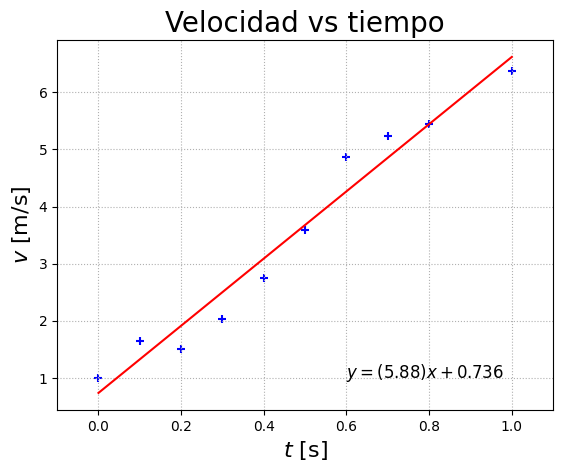
\includegraphics[height=2.6in,width=3.0in]{figuras/fig13}  
\label{figdatos2}
\end{center}
\end{figure}

El siguiente paso es calcular $\Delta b$ y $\Delta m$

\begin{lstlisting}[language=Python] 
# Escribimos las sumatorias para calcular Sy
Sum_d= Sum_y-b-m*Sum_x
Sy=sqrt(Sum_d/(n-2))
print(n,',', Sum_d,',', Sy)
\end{lstlisting}
\begin{tcolorbox}[width=\textwidth,colback={ghostwhite}]   
{\small 
10 , 6.625519480519479 , 0.9100494135292516
}
\end{tcolorbox}

Los respectivos errores se obtienen de las ecuaciones (\ref{Delm}) y (\ref{Delb}) 

\begin{lstlisting}[language=Python] 
Dm= (n/((n*Sum_xx-Sum_x**2)))**(1/2)*Sy
Db= (Sum_xx/((n*Sum_xx-Sum_x**2)))**(1/2)*Sy
print('Dm=', Dm, ',', 'Db=',Db)
\end{lstlisting}
\begin{tcolorbox}[width=\textwidth,colback={ghostwhite}]   
{\small 
Dm= 0.9467362111662778 , Db= 0.5219943236034063
}
\end{tcolorbox}

Por lo tanto:
$$
v= 5.88 t + 0.736 \,\, \mathrm{m/s}
$$
donde: $m=5.88 \pm 0.95$ y $b=0.74 \pm 0.52$.



\section{An\'alisis Gr\'afico de Funciones}
En el an\'alisis de un experimento generalmente se dispone de un conjunto de datos que de acuerdo a la teor\'ia del fen\'omeno en estudio debe corresponder a una cierta ley f\'isica. ley  que se expresa mediante una ecuaci\'on matem\'atica.  Este an\'alisis se puede lograr graficando los valores experimentales que seguramente seguir\'an una cierta curva que corresponde a la tendencia de los puntos.  La idea es comparar la forma de la curva obtenida por la mediciones con la predicha por la teor\'ia. Si la comparaci\'on muestran la misma tendencia se concluye que esto es una comprobaci\'on experimental de la teor\'ia considerada.

Como es m\'as f\'acil obtener la informaci\'on de un gr\'afico lineal, entonces se procede a elegir convenientemente las variables de modo de obtener una funci\'on lineal. A continuaci\'on se mostrar\'a como algunas de las funciones m\'as conocidas pueden ser llevadas a un gr\'afico lineal.

\subsection{Funci\'on exponencial}
Dada la funci\'on 
\begin{equation}
y(x)=k a^{b x}
\label{funexp}
\end{equation}
donde $k, a$ y $b$ son constantes. Si  $b>0$  la exponencial es creciente, mientras que si si $b < 0$, la exponencial es decreciente. Notemos  que en $x=0$, $y=k$, por lo que $k$ resulta ser la ordenada al origen, es decir, la curva intercepta al eje de las ordenadas en el punto $(0, k)$.

Tomando logaritmos se tiene:
\begin{equation}
\log (y)=b \log(a) x +\log (k)
\label{funexplin}
\end{equation}
Recordemos que si por ejemplo $a=10$ debemos tomar  logaritmo en base diez. 

Si hacemos una gr\'afica directamente $\log y$ en funci\'on de $x$  se obtendr\'a una recta, pero para ello habr\'ia que calcular los logaritmos de $y$. Este c\'alculo puede ser evitado usando un papel especial llamado papel semi-logar\'itmico, en el cual uno de los ejes tiene las divisiones proporcionales a los logaritmos decimales y el otro es lineal. 

En la escala logar\'itmica existen ciclos, donde un ciclo corresponde al conjunto de n\'umeros entre dos potencias de diez (1 a $10; 10$ a $100; 100$ a 1000 \'o 0,1 a 1; etc.).

El gr\'afico de la funci\'on $y=k a^{bx}$ es una recta porque la ecuaci\'on (\ref{funexplin}) puede ser escrita como
$$
u=m x+v \,,
$$
donde: $u =\log(y)$,  $m =b \log(a)$ y  $v=\log (k)$.

Para calcular la pendiente de la recta hay que considerar que se est\'a trabajando con logaritmos:
$$
\text {pendiente}=m=\frac{u_2-u_1}{x_2-x_1}  =\frac{\log y_2-\log y_1}{x_2-x_1}=b \log a
$$

Es de hacer notar que al graficar en papel semi-logar\'itmico y llevar los valores en la escala logar\'itmica, se llevan directamente los n\'umeros a la escala y no se calculan los logaritmos, pero al calcular la pendiente si es necesario hacerlo. Adem\'as si se est\'a utilizando papel semi-logar\'itmico, $k$ es el corte de la recta en $x=0$.

En las siguientes lineas de c\'odigo podemos interpretar lo expuesto anteriormente tomando la funci\'on exponencial siguiente:
$$
y = 5\cdot 10^{\frac{x}{3}}
$$
cuya gr\'afica la podemoa hacer de la manera siguiente
\begin{lstlisting}[language=Python] 
x = arange(10)
y = 5*10**(1/3*x)
plt.plot(x, y, 'o')
plt.show()
\end{lstlisting}
\begin{figure}[h]
\begin{center}
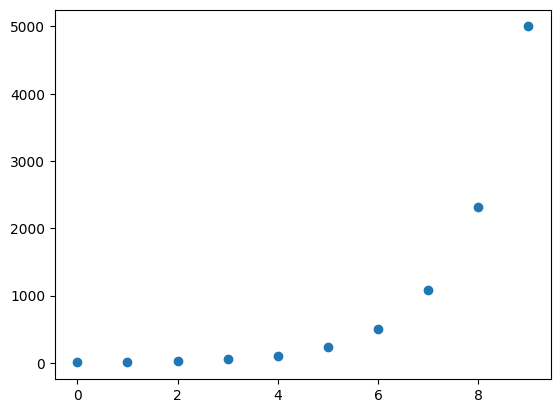
\includegraphics[height=2.4in,width=2.9in]{figuras/fig14}  
\label{figexp1}
\end{center}
\end{figure}

Ahora la funci\'on lineal pero en escala logar\'itmica
\begin{lstlisting}[language=Python] 
plt.plot(x, y, '-o')
plt.yscale("log")
plt.show()
\end{lstlisting}
\begin{figure}[h]
\begin{center}
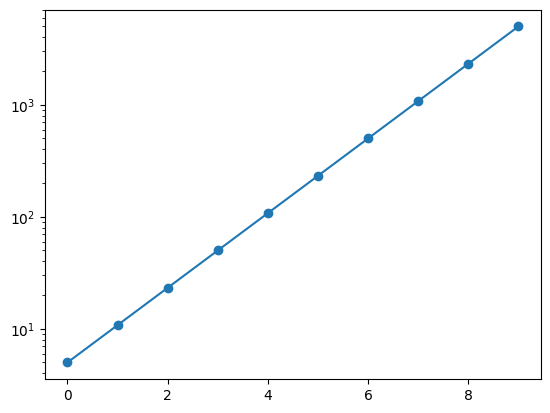
\includegraphics[height=2.4in,width=2.9in]{figuras/fig15}  
\label{figexp1lin}
\end{center}
\end{figure}

\newpage
\subsection{Funci\'on potencial}
Dada la funci\'on:
\begin{equation}
y= c x^m
\label{funpot}
\end{equation}
donde $m$ y $c$ son constantes. 

Tomando logaritmos decimales  se tiene:
\begin{equation}
\log (y)=m \log (x)+\log (c)
\label{funpotlin}
\end{equation}

Si se hace una gr\'afica directamente $\log y$ en funci\'on de $\log x$ se obtendr\'a una recta, pero habr\'ia que calcular los logaritmos decimales de $y$ y de $x$. Esto se puede  evitar  usando un papel especial llamado papel logar\'itmico (com\'unmente llamado $\log-\log$ ), el cual tiene ambas escalas proporcionales a los logaritmos decimales.

El gr\'afico de la funci\'on $y=c x^m$ es una recta porque la ecuaci\'on (\ref{funpotlin}) se puede escribir como:
$$
v=m u+k \,,
$$
donde: $v =\log(y) $, $u=\log(x) $ y $k=\log(c)$

La pendiente $m$ de la recta est\'a dada por:
$$
m =\frac{v_2-v_1}{u_2-u_1}  =\frac{\log y_2-\log y_1}{\log x_2-\log x_1}=\frac{\log \left(\frac{y_2}{y_1}\right)}{\log \left(\frac{x_2}{x_1}\right)}
$$
y $c$ representa el corte de la recta en $x=1(\log 1=0)$.

Consideremos la  funci\'on potencial siguiente:
$$
y = 8\ x^{3}
$$

Procedemos a realizar su gr\'afica:
\begin{lstlisting}[language=Python] 
x = arange(20)
y = 8*x**(3)
plt.plot(x, y, '*')
plt.show()
\end{lstlisting}
\begin{figure}[h]
\begin{center}
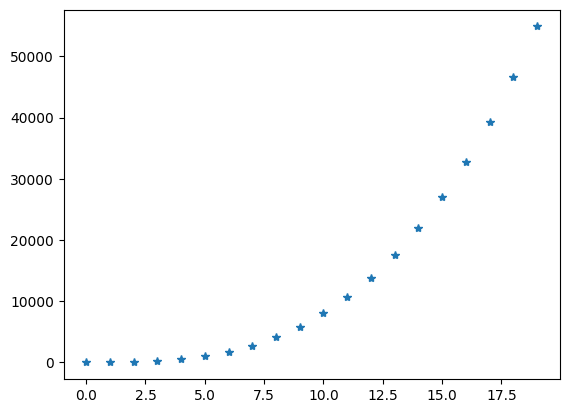
\includegraphics[height=2.4in,width=2.9in]{figuras/fig16}  
\label{figexp1}
\end{center}
\end{figure}
\newpage

Ahora la funci\'on lineal pero en escala log-log
\begin{lstlisting}[language=Python] 
plt.plot(x, y, '-*')
plt.xscale("log")
plt.yscale("log")
plt.show()
\end{lstlisting}
\begin{figure}[h]
\begin{center}
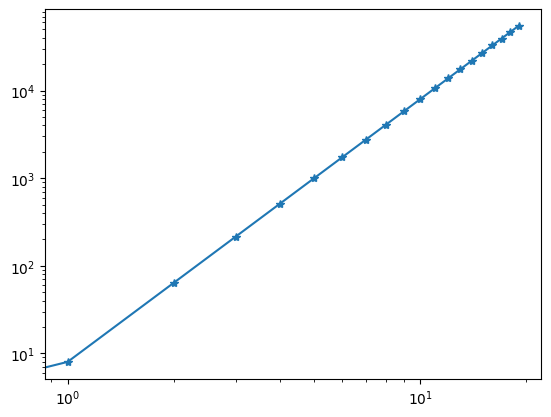
\includegraphics[height=2.4in,width=2.9in]{figuras/fig17}  
\label{figexp1lin}
\end{center}
\end{figure}



